\documentclass[tikz,border=15pt]{standalone}
\usepackage{amsmath,amssymb}
\usepackage{tikz}
\usetikzlibrary{arrows.meta,calc,positioning,shapes.geometric,shapes.misc,patterns}

% Exact color scheme
\definecolor{genyellow}{RGB}{255,232,0}
\definecolor{ibrblue}{RGB}{205,225,252}
\definecolor{ibrborder}{RGB}{120,165,230}
\definecolor{storegreen}{RGB}{225,248,225}
\definecolor{storeborder}{RGB}{50,150,50}
\definecolor{textgreen}{RGB}{0,150,70}
\definecolor{textblue}{RGB}{0,102,204}

\begin{document}
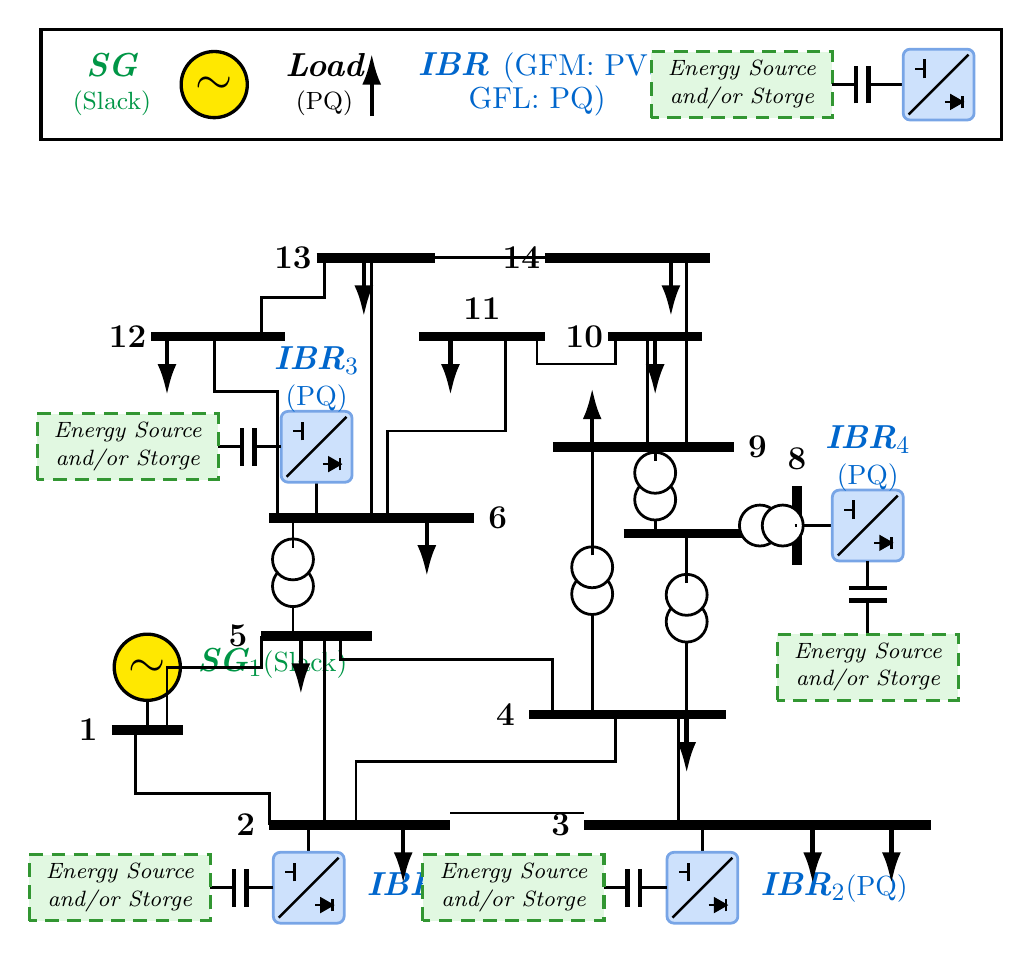
\begin{tikzpicture}[
  >=Latex,
  line width=1.0pt,
  font=\sffamily\fontsize{10pt}{12pt}\selectfont,
  bus/.style={line width=3.5pt, draw=black, line cap=square},
  loadarr/.style={-{Latex[length=4.0mm, width=2.4mm]}, line width=1.6pt, draw=black},
  txcirc/.style={circle, draw=black, line width=1.0pt, minimum size=5.2mm, inner sep=0pt, fill=white}
]

% Macro / Pic for Converter Symbol (Clean IGBT + Diode inside blue box)
\tikzset{
  converter/.pic={
    \draw[fill=ibrblue, draw=ibrborder, rounded corners=2.5pt, line width=1.0pt] (-0.45,-0.45) rectangle (0.45,0.45);
    % Diagonal line
    \draw[line width=0.9pt] (-0.38,-0.38) -- (0.38,0.38);
    % Transistor (top-left)
    \draw[line width=0.9pt] (-0.18,0.08) -- (-0.18,0.32);
    \draw[line width=0.9pt] (-0.30,0.20) -- (-0.18,0.20);
    % Diode (bottom-right)
    \draw[line width=0.8pt] (0.08,-0.22) -- (0.30,-0.22);
    \draw[line width=0.8pt, fill=black] (0.16,-0.30) -- (0.16,-0.14) -- (0.30,-0.22) -- cycle;
    \draw[line width=0.9pt] (0.30,-0.30) -- (0.30,-0.14);
  },
  capacitor_h/.pic={
    \draw[line width=1.0pt] (-0.28,0) -- (-0.08,0);
    \draw[line width=1.6pt] (-0.08,-0.24) -- (-0.08,0.24);
    \draw[line width=1.6pt] (0.08,-0.24) -- (0.08,0.24);
    \draw[line width=1.0pt] (0.08,0) -- (0.28,0);
  },
  capacitor_v/.pic={
    \draw[line width=1.0pt] (0,-0.28) -- (0,-0.08);
    \draw[line width=1.6pt] (-0.24,-0.08) -- (0.24,-0.08);
    \draw[line width=1.6pt] (-0.24,0.08) -- (0.24,0.08);
    \draw[line width=1.0pt] (0,0.08) -- (0,0.28);
  },
  storagebox/.pic={
    \draw[fill=storegreen, draw=storeborder, line width=1.1pt, dash pattern=on 5pt off 3pt] (-1.15,-0.42) rectangle (1.15,0.42);
    \node[align=center, font=\fontsize{8.5pt}{10pt}\selectfont\itshape, text=black] at (0,0) {Energy Source\\and/or Storge};
  }
}

% =========================================================================
% TOP LEGEND BOX
% =========================================================================
\draw[line width=1.3pt] (-1.2, 10.0) rectangle (11.0, 11.4);

% SG legend
\node[text=textgreen, font=\bfseries\itshape\fontsize{12pt}{14pt}\selectfont, align=center] at (-0.3, 10.7) {SG\\[-2pt]{\normalfont\fontsize{9.5pt}{11pt}\selectfont(Slack)}};
\draw[fill=genyellow, draw=black, line width=1.2pt] (1.0, 10.7) circle (0.42cm);
\node[font=\bfseries\fontsize{17pt}{17pt}\selectfont] at (1.0, 10.68) {$\sim$};

% Load legend
\node[font=\bfseries\itshape\fontsize{12pt}{14pt}\selectfont, align=center] at (2.4, 10.7) {Load\\[-2pt]{\normalfont\fontsize{9.5pt}{11pt}\selectfont(PQ)}};
\draw[loadarr] (3.0, 10.3) -- (3.0, 11.1);

% IBR legend
\node[text=textblue, font=\bfseries\itshape\fontsize{12pt}{14pt}\selectfont, align=center] at (5.1, 10.7) {IBR {\normalfont\fontsize{10.5pt}{12pt}\selectfont(GFM: PV,}\\[-2pt]{\normalfont\fontsize{10.5pt}{12pt}\selectfont GFL: PQ)}};

% Storage + Cap + Converter legend
\pic at (7.7, 10.7) {storagebox};
\draw[line width=1.0pt] (8.85, 10.7) -- (8.95, 10.7);
\pic at (9.23, 10.7) {capacitor_h};
\draw[line width=1.0pt] (9.51, 10.7) -- (9.75, 10.7);
\pic at (10.2, 10.7) {converter};


% =========================================================================
% BUSES DEFINITIONS
% =========================================================================
% Bus 1
\draw[bus] (-0.3, 2.5) -- (0.6, 2.5);
\node[font=\bfseries\fontsize{12pt}{12pt}\selectfont] at (-0.6, 2.5) {1};

% Bus 2
\draw[bus] (1.7, 1.3) -- (4.0, 1.3);
\node[font=\bfseries\fontsize{12pt}{12pt}\selectfont] at (1.4, 1.3) {2};

% Bus 3 (Single continuous bar)
\draw[bus] (5.7, 1.3) -- (10.1, 1.3);
\node[font=\bfseries\fontsize{12pt}{12pt}\selectfont] at (5.4, 1.3) {3};

% Bus 4
\draw[bus] (5.0, 2.7) -- (7.5, 2.7);
\node[font=\bfseries\fontsize{12pt}{12pt}\selectfont] at (4.7, 2.7) {4};

% Bus 5
\draw[bus] (1.6, 3.7) -- (3.0, 3.7);
\node[font=\bfseries\fontsize{12pt}{12pt}\selectfont] at (1.3, 3.7) {5};

% Bus 6
\draw[bus] (1.7, 5.2) -- (4.3, 5.2);
\node[font=\bfseries\fontsize{12pt}{12pt}\selectfont] at (4.6, 5.2) {6};

% Bus 7
\draw[bus] (6.2, 5.0) -- (8.0, 5.0);
\node[font=\bfseries\fontsize{12pt}{12pt}\selectfont] at (8.3, 5.0) {7};

% Bus 8 (Vertical busbar)
\draw[bus] (8.4, 4.6) -- (8.4, 5.6);
\node[font=\bfseries\fontsize{12pt}{12pt}\selectfont] at (8.4, 5.95) {8};

% Bus 9
\draw[bus] (5.3, 6.1) -- (7.6, 6.1);
\node[font=\bfseries\fontsize{12pt}{12pt}\selectfont] at (7.9, 6.1) {9};

% Bus 10
\draw[bus] (6.0, 7.5) -- (7.2, 7.5);
\node[font=\bfseries\fontsize{12pt}{12pt}\selectfont] at (5.7, 7.5) {10};

% Bus 11
\draw[bus] (3.6, 7.5) -- (5.2, 7.5);
\node[font=\bfseries\fontsize{12pt}{12pt}\selectfont] at (4.4, 7.85) {11};

% Bus 12
\draw[bus] (0.2, 7.5) -- (1.9, 7.5);
\node[font=\bfseries\fontsize{12pt}{12pt}\selectfont] at (-0.1, 7.5) {12};

% Bus 13
\draw[bus] (2.3, 8.5) -- (3.8, 8.5);
\node[font=\bfseries\fontsize{12pt}{12pt}\selectfont] at (2.0, 8.5) {13};

% Bus 14
\draw[bus] (5.2, 8.5) -- (7.3, 8.5);
\node[font=\bfseries\fontsize{12pt}{12pt}\selectfont] at (4.9, 8.5) {14};


% =========================================================================
% GENERATOR SG1 (at Bus 1)
% =========================================================================
\draw[fill=genyellow, draw=black, line width=1.2pt] (0.15, 3.3) circle (0.42cm);
\node[font=\bfseries\fontsize{17pt}{17pt}\selectfont] at (0.15, 3.28) {$\sim$};
\draw[line width=1.1pt] (0.15, 2.88) -- (0.15, 2.5);
\node[text=textgreen, font=\bfseries\itshape\fontsize{13pt}{15pt}\selectfont, anchor=west] at (0.65, 3.35) {SG$_1$\\[-2pt]{\normalfont\fontsize{10pt}{11pt}\selectfont(Slack)}};


% =========================================================================
% DUAL-MODE IBRS + CAPACITORS + STORAGE
% =========================================================================

% IBR1 (at Bus 2)
\draw[line width=1.1pt] (2.2, 1.3) -- (2.2, 0.95);
\pic at (2.2, 0.5) {converter};
\draw[line width=1.0pt] (1.75, 0.5) -- (1.61, 0.5);
\pic at (1.33, 0.5) {capacitor_h};
\draw[line width=1.0pt] (1.05, 0.5) -- (0.95, 0.5);
\pic at (-0.2, 0.5) {storagebox};
\node[text=textblue, font=\bfseries\itshape\fontsize{13pt}{15pt}\selectfont, anchor=west] at (2.8, 0.5) {IBR$_1$\\[-2pt]{\normalfont\fontsize{10pt}{11pt}\selectfont(PQ)}};

% IBR2 (at Bus 3)
\draw[line width=1.1pt] (7.2, 1.3) -- (7.2, 0.95);
\pic at (7.2, 0.5) {converter};
\draw[line width=1.0pt] (6.75, 0.5) -- (6.61, 0.5);
\pic at (6.33, 0.5) {capacitor_h};
\draw[line width=1.0pt] (6.05, 0.5) -- (5.95, 0.5);
\pic at (4.8, 0.5) {storagebox};
\node[text=textblue, font=\bfseries\itshape\fontsize{13pt}{15pt}\selectfont, anchor=west] at (7.8, 0.5) {IBR$_2$\\[-2pt]{\normalfont\fontsize{10pt}{11pt}\selectfont(PQ)}};

% IBR3 (at Bus 6)
\draw[line width=1.1pt] (2.3, 5.2) -- (2.3, 5.65);
\pic at (2.3, 6.1) {converter};
\draw[line width=1.0pt] (1.85, 6.1) -- (1.71, 6.1);
\pic at (1.43, 6.1) {capacitor_h};
\draw[line width=1.0pt] (1.15, 6.1) -- (1.05, 6.1);
\pic at (-0.1, 6.1) {storagebox};
\node[text=textblue, font=\bfseries\itshape\fontsize{13pt}{15pt}\selectfont, align=center] at (2.3, 6.95) {IBR$_3$\\[-2pt]{\normalfont\fontsize{10pt}{11pt}\selectfont(PQ)}};

% IBR4 (at Bus 8)
\draw[line width=1.1pt] (8.4, 5.1) -- (8.85, 5.1);
\pic at (9.3, 5.1) {converter};
\draw[line width=1.0pt] (9.3, 4.65) -- (9.3, 4.51);
\pic at (9.3, 4.23) {capacitor_v};
\draw[line width=1.0pt] (9.3, 3.95) -- (9.3, 3.72);
\pic at (9.3, 3.3) {storagebox};
\node[text=textblue, font=\bfseries\itshape\fontsize{13pt}{15pt}\selectfont, align=center] at (9.3, 5.95) {IBR$_4$\\[-2pt]{\normalfont\fontsize{10pt}{11pt}\selectfont(PQ)}};


% =========================================================================
% SYSTEM LOADS
% =========================================================================
% Load Bus 2
\draw[loadarr] (3.4, 1.3) -- (3.4, 0.55);
% Load Bus 3 (2 loads)
\draw[loadarr] (8.6, 1.3) -- (8.6, 0.55);
\draw[loadarr] (9.6, 1.3) -- (9.6, 0.55);
% Load Bus 4
\draw[loadarr] (7.0, 2.7) -- (7.0, 1.95);
% Load Bus 5
\draw[loadarr] (2.1, 3.7) -- (2.1, 2.95);
% Load Bus 6
\draw[loadarr] (3.7, 5.2) -- (3.7, 4.45);
% Load Bus 9 (Points UP!)
\draw[loadarr] (5.8, 6.1) -- (5.8, 6.85);
% Load Bus 10
\draw[loadarr] (6.6, 7.5) -- (6.6, 6.75);
% Load Bus 11
\draw[loadarr] (4.0, 7.5) -- (4.0, 6.75);
% Load Bus 12
\draw[loadarr] (0.4, 7.5) -- (0.4, 6.75);
% Load Bus 13
\draw[loadarr] (2.9, 8.5) -- (2.9, 7.75);
% Load Bus 14
\draw[loadarr] (6.8, 8.5) -- (6.8, 7.75);


% =========================================================================
% TRANSFORMERS (Two interlocking circles)
% =========================================================================
% Transformer 5-6 (Vertical)
\draw[line width=1.0pt] (2.0, 3.7) -- (2.0, 4.18);
\node[txcirc] at (2.0, 4.33) {};
\node[txcirc] at (2.0, 4.67) {};
\draw[line width=1.0pt] (2.0, 4.82) -- (2.0, 5.2);

% Transformer 4-9 (Vertical)
\draw[line width=1.0pt] (5.8, 2.7) -- (5.8, 4.08);
\node[txcirc] at (5.8, 4.23) {};
\node[txcirc] at (5.8, 4.57) {};
\draw[line width=1.0pt] (5.8, 4.72) -- (5.8, 6.1);

% Transformer 7-9 (Vertical)
\draw[line width=1.0pt] (6.6, 5.0) -- (6.6, 5.28);
\node[txcirc] at (6.6, 5.43) {};
\node[txcirc] at (6.6, 5.77) {};
\draw[line width=1.0pt] (6.6, 5.92) -- (6.6, 6.1);

% Transformer 4-7 (Vertical)
\draw[line width=1.0pt] (7.0, 2.7) -- (7.0, 3.5) -- (7.0, 3.73);
\node[txcirc] at (7.0, 3.88) {};
\node[txcirc] at (7.0, 4.22) {};
\draw[line width=1.0pt] (7.0, 4.37) -- (7.0, 5.0);

% Transformer 7-8 (Horizontal)
\draw[line width=1.0pt] (7.7, 5.0) -- (7.7, 5.1) -- (7.75, 5.1);
\node[txcirc] at (7.93, 5.1) {};
\node[txcirc] at (8.22, 5.1) {};
\draw[line width=1.0pt] (8.37, 5.1) -- (8.4, 5.1);


% =========================================================================
% TRANSMISSION LINES
% =========================================================================
% Line 1-2
\draw[line width=1.0pt] (0.0, 2.5) -- (0.0, 1.7) -- (1.7, 1.7) -- (1.7, 1.3);

% Line 1-5
\draw[line width=1.0pt] (0.4, 2.5) -- (0.4, 3.3) -- (1.6, 3.3) -- (1.6, 3.7);

% Line 2-3
\draw[line width=1.0pt] (4.0, 1.45) -- (5.7, 1.45);

% Line 2-4
\draw[line width=1.0pt] (2.8, 1.3) -- (2.8, 2.1) -- (6.1, 2.1) -- (6.1, 2.7);

% Line 2-5
\draw[line width=1.0pt] (2.4, 1.3) -- (2.4, 3.7);

% Line 3-4
\draw[line width=1.0pt] (6.9, 1.3) -- (6.9, 2.7);

% Line 4-5
\draw[line width=1.0pt] (5.3, 2.7) -- (5.3, 3.4) -- (2.6, 3.4) -- (2.6, 3.7);

% Line 6-11
\draw[line width=1.0pt] (3.2, 5.2) -- (3.2, 6.3) -- (4.7, 6.3) -- (4.7, 7.5);

% Line 6-12
\draw[line width=1.0pt] (1.8, 5.2) -- (1.8, 6.8) -- (1.0, 6.8) -- (1.0, 7.5);

% Line 6-13
\draw[line width=1.0pt] (3.0, 5.2) -- (3.0, 8.5);

% Line 10-11
\draw[line width=1.0pt] (5.1, 7.5) -- (5.1, 7.15) -- (6.1, 7.15) -- (6.1, 7.5);

% Line 9-10
\draw[line width=1.0pt] (6.5, 6.1) -- (6.5, 7.5);

% Line 9-14
\draw[line width=1.0pt] (7.0, 6.1) -- (7.0, 8.5);

% Line 12-13
\draw[line width=1.0pt] (1.6, 7.5) -- (1.6, 8.0) -- (2.4, 8.0) -- (2.4, 8.5);

% Line 13-14
\draw[line width=1.0pt] (3.8, 8.5) -- (5.2, 8.5);

\end{tikzpicture}
\end{document}
